\section{The problem}\label{problem}

%0.5 page

%TODO Renan: Problem

Hydropower runner's blades are typically eroded by cavitation and abrasion
phenomena, resulting in hydraulic profile deformation, thus efficiency
reduction. The High Velocity Oxygen Fuel (HVOF) coating is a preventive
solution for erosion, and creates a lamellar structure, increasing
power generation efficiency. 

The runner's blade HVOF process consists of spraying coating particles
by an 8~kg spray gun. To achieve the best coating layer, the spray gun should be at a
fixed 210~mm to 240~mm distance and $90^o \pm 30^o$ angle, in respect
to the metallic surface plane of the blade; the gun should move with 40 m/s
speed along the blade; and the precision (or coating step) should be 3~mm for a
regular full blade cover, due to the 5~mm diameter of the gun's output (flame)
\cite{li2002effect}.

Regarding the requirements, the common solution for \textit{ex situ} HVOF
coating is a robotic manipulator with a blade-sized workspace in a fixed
position. However, \textit{in situ} runner's blade HVOF coating represents
great technological challenges. The robotic system must overcome
turbine's environmental aspects, such as, the constrained space and turbine's
access, the slippery and sloping floor, and the unfriendly atmospheric
conditions. Therefore, a large-sized industrial robotic manipulator is not
suitable for the operation.

The Jirau's dam is the case study of EMMA. The plant has horizontal
axis bulb type turbines. The turbine's points of interest for the
development of EMMA are: 1) the variable pitch propeller, or Kaplan
\textbf{blades}, which are approximately 2500~mm tall and 3000~mm wide; 2) the
variable pitch guide vanes, or \textbf{wicket gates}; 3) the \textbf{runner
area}; 4) the \textbf{draft tube}; and 5) the 800~mm access for regular
maintenance, or \textbf{hatch}. A 3D CAD model of the turbine was built with
SolidWorks\raisebox{1ex}{\textregistered} for simulation and solution analysis
(Fig.~\ref{fig::ambiente3d}).
 
 %TODO Renan/Estevão: alterar figura
\begin{figure}[h!]
\centering
	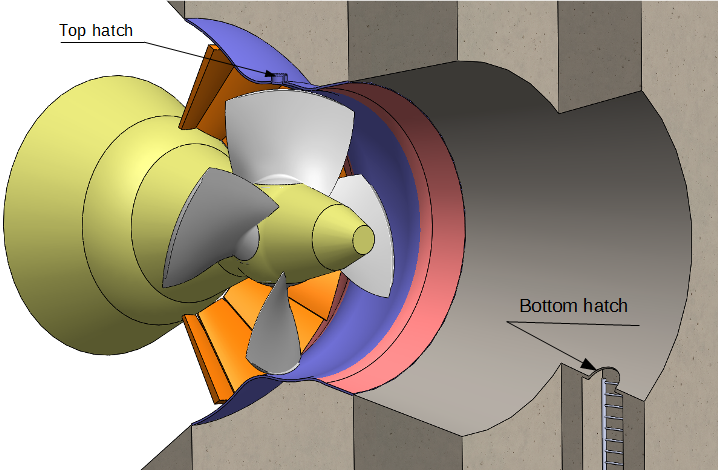
\includegraphics[width=\columnwidth]{figs/problem/ambiente_3d.PNG} 
	\caption{Elements of the Jirau's hydropower turbine in a 3D CAD model.}
	\label{fig::ambiente3d}
\end{figure}


As the runner can be manually rotated, the main problem and objective of the
proposed robotic system is to hard coat the two sides of one blade. The
robotic system must comply with the HVOF requirements, it must overcome the
constraints and logistical challenges of the environment, and operate in
autonomously mode. 

